\documentclass[12pt]{article}

\usepackage[
  paper=a4paper,
  left=12.5mm,
  right=25mm,
  top=25mm,
  bottom=40mm,
  bindingoffset=10mm]{geometry}		% page and binding margins can be adjust here
  
\usepackage{apacite} 				% % literature-References: American Psycholog. Assoc.
\usepackage{natbib}					

\setcitestyle{round,aysep={}} 		% indexation in (round) parentheses, between the author year
%\usepackage[latin1]{inputenc} 		% mutated vowel (Umlaute) in the text
\usepackage[english]{babel}				% orthography
\usepackage[T1]{fontenc}
\usepackage{lmodern}				% font family
\usepackage{microtype}				% for micro typography (for a better typeface)
\usepackage{blindtext}
\usepackage{graphicx} 				% for including graphs (pdf,png - but do avoid jpg)
\graphicspath{{./Graphics/}}          % path to the pictures

\usepackage{url}					%  formatting URL (e.g. in the literature) 
\usepackage[colorlinks,linkcolor=black,citecolor=black,urlcolor=black]{hyperref} 				% For hperlinks in PDF-documents   
  
\usepackage{tabularx} 				% for a better configuration of tables
\usepackage{longtable} 		
\usepackage{multicol}				
\usepackage{multirow}
\usepackage{booktabs}
\usepackage{tabularx}
\usepackage{xcolor}
\usepackage{varioref}
		
\usepackage[active]{srcltx}

\usepackage{listings}				% algorithm

\usepackage{mdwlist}				% lists

\usepackage{setspace} 				% setting of the lines (rows)
\newtheorem{mydef}{Merksatz}  		% if examples or mnemotechnic verses are used with continuous numeration 
\newtheorem{bsp}{Beispiel}

\usepackage{todonotes}				% for the creation of ToDos in the editor
\usepackage{lscape}					% for the rotation of pages
\usepackage{amsmath}				% for the writting of mathematical formula
\usepackage{calc}
\usepackage{footnote}				% footnotes
\usepackage{tablefootnote}			% footnotes in tables
\hyphenation{voll-st\"andigen}		% for defining word devisions globally

\setcounter{tocdepth}{2}			% levels which are displayed in the table of contents








\section{Introduction}
TESTHELLO This is a template for the seminar paper. Right now, the template contains different examples that you might find helpful once you write down your results in \LaTeX, a software system for document preparation. A lot of useful information can be found at the \href{https://www.overleaf.com/learn/latex/Creating_a_document_in_LaTeX}{\textbf{Overleaf}}-Homepage. Overleaf also provides a convenient online editor that is ideal to collaborate on joint projects and access your project from different devices. Feel free to use it in your group!


 Other open source editors to work on your device offline are available on the internet as well. An easy way to get started is the \href{https://miktex.org/download}{\underline{MikTeX-distribution}}. Once you installed MikTeX, a nice open source editor is \href{https://www.texstudio.org/}{\underline{TeXstudio}}. \\
\LaTeX is widely used in academia. It is especially common in quantitative fields because writing and formatting equations, graphs and tables is very convenient. It is also easy to insert graphs, create tables and (most importantly!) correctly cite your sources. \\
To help you get a feeling for \LaTeX, this template is structured in the following way: Section \ref{sec:math_mode} will introduce how to write equations while graphs, tables and citations are discussed in \ref{sec:results}. Like any scientific paper the last section \ref{sec:conclusion} is the conclusion that provides a high level summary of the most important findings of the paper!

\section{Methodology}\label{sec:math_mode}
The mathmode allows to easily write equations, using various mathematical operators, greek letters, symbols and formatting environments. In the following paragraphs will introduce the most important commands and functions based on different examples. This is done using \textbf{math mode}.\footnote{to highlight words or phrases, it is also possible to write text in \textit{italic}, \textbf{bold} or \textsf{sans serif}.}
\subsection{Some examples for math mode}
To include mathematical expressions like $x = 7$ in the written text use one \$-sign to start and close the . Two \$-signs indent the expression on a new line $$a^2 + b^2 = c^2.$$ Greek letters can be written using a \texttt{\textbackslash} and the greek letter spelled out. For example, the change of a variable $\zeta_t$ is often denoted as
$$ \Delta \zeta_t = \zeta_t - \zeta_{t-1}$$
 Equations can also be numerated and labeled using the command \texttt{\textbackslash begin\{equation\}} and \texttt{\textbackslash end\{equation\}} For example equation (\ref{eq:nd}) shows the distribution function $F(x)$ of a normal distributed random variable $x \sim \mathcal{N}(\mu,\sigma^2)$ that is given as
\begin{equation}\label{eq:nd}
	F(x) = \frac{1}{\sqrt{2\pi \sigma^2}}\int_{-\infty}^{x}e^{-\frac{(x-\mu)^2}{2\sigma^2}}
\end{equation}
Using \texttt{equation*} suppresses the numbering.
\begin{equation*}
x_t = \mu_t + \sum_{i=0}^{\infty}\psi_i u_{t-i}
\end{equation*}
The same holds for \texttt{\textbackslash begin\{align\}} and \texttt{\textbackslash end\{align\}} which can be used to align several expressions (note that \texttt{align} numbers every line).
\begin{align*}
x_t &= c + \alpha x_{t-1} + u_t \\
x_t &= c + \alpha Lx_t + u_t  \\
(1-\alpha L)x_t &= c + u_t \\
x_t &= \frac{c}{1-\alpha} + \sum_{i=0}^{\infty}\alpha^ix_{t-i} \quad (\longrightarrow \text{Wold Representation})
\end{align*}
The \texttt{\&}-sign indicates where the expressions should be aligned and \texttt{\textbackslash \textbackslash} marks the line breaks.
Adjusting the size of brackets works with the commands \texttt{\textbackslash left} and \texttt{\textbackslash right} in front of the brackets. For example, for a Cobb-Douglas function $f(L,K) = L^{\alpha}K^{(1-\alpha)}$ it holds that
\begin{equation}
	\frac{\partial f(L,K)}{\partial L} = \alpha \left[\frac{K}{L}\right]^{(1-\alpha)} \quad \text{and} \quad \frac{\partial f(L,K)}{\partial K} = (1-\alpha)\left[\frac{L}{K}\right]^{\alpha} \quad \forall \; 0 < \alpha < 1
\end{equation}


\section{Results}\label{sec:results}
\LaTeX also provides an environment to create tables, for example to create customized regression outputs or summary statistics. Additionally, it provides an easy and efficient way to cite other sources using BibTeX. Examples for both features are given in the next subsections. 
\subsection{Example: Figures and Tables}

Table \ref{tab:exmpl1} is an example of how a table is generated and can be included in the text.
\begin{table}[h]
	\centering
	\begin{tabular}{l|c r}
		\hline
		\textbf{Left} & \textbf{Middle} & \textbf{Right} \\ \hline \hline
		text & text & text \\ 
		in these & in these & in these \\ 
		cells & cells & cells \\
		will be & will be & will be \\
		left aligned & centered & right aligned \\ \hline
	\end{tabular}
	\caption{Example how to create and insert tables}
	\label{tab:exmpl1}
\end{table} 
To draw vertical lines use $|$ in the \texttt{\textbackslash begin\{\}} command. For horizontal lines use \texttt{\textbackslash hline}. The \texttt{\&}-signs indicate cells and \texttt{\textbackslash \textbackslash} marks a line break. For complicated or large tables, there are also convenient \href{https://www.tablesgenerator.com/}{\textbf{websites}} that can help you generate the appropriate \LaTeX-Code.
It is always useful to illustrate your method, simulations, data set or other results using figures and plots. This section shows how to include and refer to them in your text in \LaTeX.
\subsection{Example Figures}
It is always useful to illustrate your method, simulations, data set or other results using figures and plots. This section shows how to include and refer to them in your text in \LaTeX.
% compared to \ref{}, \vref{} autmatically adds the page that the grafic or table apprears to your text. It is quite convenient, but comes at the risk that sometimes the sentences are no longer gramatically correct. 
Figure \vref{fig:bsp1} is an example of how an image file can be included in the text. 
\begin{figure}[h!]
	\centering
	
\includegraphics[width=0.7\textwidth]{./Graphics/bsp1.png}
	\caption{Example how to insert graphics}
	\label{fig:bsp1}
\end{figure}
It is important that the relevant file is stored in the folder Graphics. The size of the figures can be controlled using the argument \texttt{width} or alternatively with the argument \texttt{scale}. 
Similar to equations, figures can be labeled using the command \texttt{\textbackslash label\{fig:fig\_name\}} and later referred to in the text using \texttt{\textbackslash ref{fig:fig\_name}}. Possible file types include but are not limited to PDF, JPG, PNG or EPS.

\subsection{Example: Citations}
To include citations, \LaTeX  uses the BibTeX tool. Before a source can be cited in a document, it has to be stored in the Bibtex-file called \texttt{sources.bib}. The file is saved in the folder \texttt{Literature} and should not be moved or renamed. Once the relevant information about the source is entered and saved in the BibTeX-file, the command \texttt{\textbackslash cite\{\}} can be used to include the citation in the document. Furthermore, the source will then automatically be displayed in the section \textbf{References} at the end of the document. Some examples that are already saved in the \texttt{sources.bib} file are \cite{brink2005anfertigung}, \cite{gopen1990science} and \cite{johnson1993get}. Note that many scientific journals provide the information about the articles in BibTeX format on their homepages so it is easy to copy and include them. Looking up sources in Google Scholar is also an easy way to find the information in BibTeX format as can be seen in Figure \ref{fig:bibtex_ex}. 
\begin{figure}[h!]
    \centering
    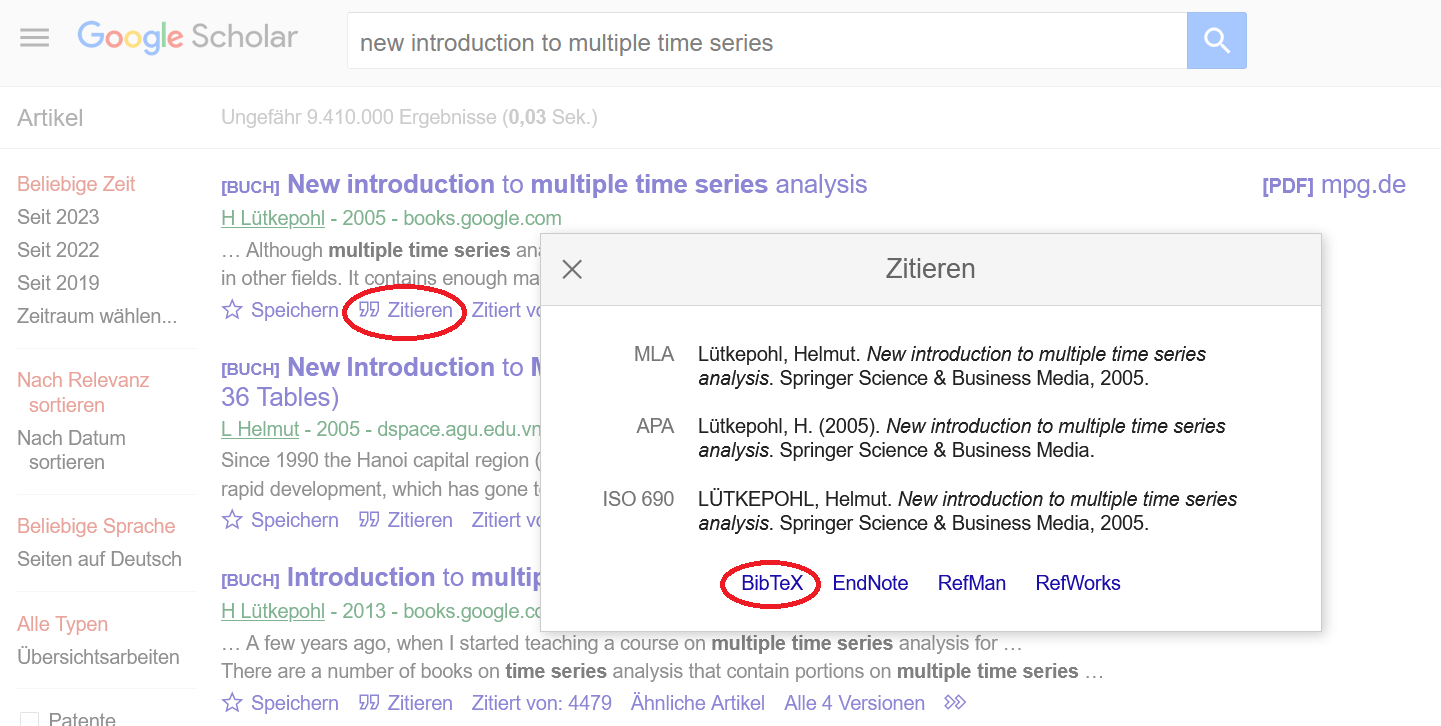
\includegraphics[scale=0.4]{Graphics/Bibtex_ex1.PNG}
    \caption{Citations in BibTeX-format can easily be obtained from Google Scholar.}
    \label{fig:bibtex_ex}
\end{figure} 

\section{Conclusion}\label{sec:conclusion}
This document provides an overview of the most important concepts and functions to work in \LaTeX, a common software system to prepare academic texts. Based on different examples, this templates illustrates how to write equations, insert graphs, create tables and consistently cite your references. \textcolor{red}{However, while \LaTeX is a powerful tool, it requires time to familiarize with the commands and debugging your code can slow you down. Consequently, this can make working in \LaTeX tedious and slow in the beginning so it is important to start writing down projects early enough!}
% -----------------------------------
\newpage
\bibliographystyle{apacite}				% by natbib in german
\bibliography{./Literature/sources}		% including literature sources
\newpage
%\newpage
\thispagestyle{empty}

\begin{large}

\vspace*{2cm}

\noindent
I declare that I have authored this thesis independently, that I have not used other than the declared sources / resources, and that I have explicitly marked all material which has been quoted either literally or by content from the used sources.

\vspace{2cm}

\noindent
Berlin, August 31, 2023
\vspace{3cm}

\hspace*{7cm}%
\dotfill\\
\hspace*{8.5cm}%
\textit{(Signature of the author)}

\end{large}
 			% % statutory declaration - "`Eidesstattliche Erklärung"'

\end{document}









This is a template for the seminar paper. Right now, the template contains different examples that you might find helpful once you write down your results in \LaTeX, a software system for document preparation. A lot of useful information can be found at the \href{https://www.overleaf.com/learn/latex/Creating_a_document_in_LaTeX}{\textbf{Overleaf}}-Homepage. Overleaf also provides a convenient online editor that is ideal to collaborate on joint projects and access your project from different devices. Feel free to use it in your group! Other open source editors to work on your device offline are available on the internet as well. An easy way to get started is the \href{https://miktex.org/download}{\underline{MikTeX-distribution}}. Once you installed MikTeX, a nice open source editor is \href{https://www.texstudio.org/}{\underline{TeXstudio}}. \\